\documentclass[letterpaper,12pt, twoside]{report}
\usepackage[utf8]{inputenc}
%\usepackage[english]{babel}
\usepackage[spanish]{babel}
\usepackage[T1]{fontenc}
\usepackage{graphicx}
\usepackage{epstopdf}
\usepackage{amssymb}
\usepackage{amsmath}
\usepackage{anysize}
\usepackage{float}
\usepackage{braket}
\usepackage{fancyhdr}
\usepackage{color}
%\usepackage{soul}
\usepackage[normalem]{ulem}
\usepackage{xcolor}
%\usepackage{CJK}
\usepackage{hyperref}
\usepackage{placeins}
\usepackage{tabularx}
\usepackage{apacite}
\usepackage{subfigure}
\usepackage{booktabs}
\usepackage{setspace}  
\usepackage{algorithm2e}
\usepackage{listings} 
\usepackage{natbib}
\lstloadlanguages{python}

%\lstset{language=python,tabsize=2}

\definecolor{codegreen}{rgb}{0,0.6,0}
\definecolor{codegray}{rgb}{0.5,0.5,0.5}
\definecolor{codepurple}{rgb}{0.58,0,0.82}
\definecolor{backcolour}{rgb}{0.95,0.95,0.92}

\lstdefinestyle{mystyle}{
    backgroundcolor=\color{white},   
    commentstyle=\color{codegreen},
    keywordstyle=\color{cyan},
    numberstyle=\tiny\color{codegray},
    stringstyle=\color{codepurple},
    basicstyle=\ttfamily\footnotesize,
    breakatwhitespace=false,         
    breaklines=true,                 
    captionpos=b,                    
    keepspaces=true,                 
    numbers=left,                    
    numbersep=5pt,                  
    showspaces=false,                
    showstringspaces=false,
    showtabs=false, 
    language=python,                 
    tabsize=1
}

\lstset{style=mystyle}

\renewcommand{\baselinestretch}{1.5}
\hypersetup{
    colorlinks=true,
    linkcolor=blue,
    anchorcolor = blue,
    filecolor=magenta,      
    urlcolor=cyan,
    citecolor = blue
}

 
%Agregar aquí los paquetes que hagan falta para su trabajo
%\usepackage[paperwidth=21.59cm ,paperheight=27.94cm,top=2.5cm,right=2.5cm,bottom=2.5cm,left=2.5cm]{geometry}
\usepackage[top=2.5cm,right=2.5cm,bottom=2.5cm,left=2.5cm]{geometry}
%\marginsize{4cm}{2.5cm}{4cm}{2.5cm}
\graphicspath{ {Figuras/} }
\setlength{\headheight}{15pt}
\pagestyle{fancy}
\fancyhf{}


\title{Desigualdad Salarial de Género en Chile 2022:\\Análisis en Condiciones Laborales Similares} %Cambiar según el título de su tesis
\author{Camilo Riquelme} %Cambiar según el nombre del autor

\makeatletter 
\let\newtitle\@title
\let\newauthor\@author
\makeatother

\AtBeginDocument{\renewcommand{\contentsname}{Contenidos}}
%\AtBeginDocument{\renewcommand{\listtablename}{List of table}}
%\AtBeginDocument{\renewcommand{\tablename}{Table}}
\begin{document}

\thispagestyle{empty}
\begin{center}
\singlespace
    
\includegraphics[scale=0.4]{logo/LOGO-UM-NEGRO-V}\\
    \vspace{0.8cm}
    \begin{large}
        \textbf{UNIVERSIDAD MAYOR}\\
        \vspace{0.3cm}
        ESCUELA DE DATA SCIENCE\\
        \vspace{1.6cm}
    \end{large}
    \begin{large}
        \textbf{\MakeUppercase{\newtitle}}\\
        \vspace{1.6cm}
    \end{large}
    \begin{large}
        PROYECTO TALLER CIENCIA DE DATOS II\\
        \vspace{1cm}

        Por\\
        \vspace{1cm}\textbf{\MakeUppercase{\newauthor}}\\
        \vspace{1.4cm}
        % \textbf{Estudiante}: Camilo Riquelme   \\
        \textbf{Profesor}:  Ariel Norambuena \\ %Modificar de acuerdo al nombre del profesor
        \vspace{0.6cm}

        \vspace{1cm}
        Santiago, Chile.\\
        Septiembre 2024 %Modificar de acuerdo al mes y el año vigentes
    \end{large}
\end{center}
 %Obligatorio

\onehalfspace
\pagenumbering{arabic}
\cfoot{\thepage}
\tableofcontents
%\addcontentsline{toc}{chapter}{\textbf{Índice de figuras}} 
%\listoffigures %Opcional: Comentar si se desea
%\addcontentsline{toc}{chapter}{\textbf{Índice de tablas}} 
%\listoftables %Opcional: Comentar si se desea
\addcontentsline{toc}{chapter}
{\textbf{Tabla de Contenidos}} 

% ESTRUCTURA PRINCIPAL
\lhead{Cap\'itulo 1}
\rhead{\newtitle}
\cfoot{\thepage}
\renewcommand{\headrulewidth}{1pt}
\renewcommand{\footrulewidth}{1pt}
\chapter{Proyecto Taller Ciencia de Datos II}

\section{Introducción}
% La introducción es la presentación clara, breve y precisa del contenido general del proyecto del Electivo de Profundización I, que invita al lector a leer el documento de forma motivante, clara y precisa. Los aspectos que debe considerar son:
%    Las motivaciones para la elección del tema.
%    Antecedentes de la problemática o necesidad abordada con el proyecto.
%    El objetivo del proyecto mencionado al final de la introducción.
%    Todas las referencias necesarias para fundamentar y validar el tema expuesto.

El presente informe aborda la problemática de la brecha salarial de género en Chile durante el año 2022, enfocándose en comparaciones bajo características laborales similares. Esta investigación se basa en un proyecto previo titulado \textit{Análisis de los Ingresos Principales en Chile: Una Perspectiva Demográfica, Regional y Comparativa con el Sueldo Mínimo}, en el cual se identificó una brecha salarial de género. Ahora, se busca ampliar y profundizar en esta brecha para comprender mejor sus causas y características. 
\begin{center}
    {\footnotesize El proyecto anterior está disponible en el siguiente \href{https://github.com/ElK1000o/Taller-Ciencia-de-Datos-I/tree/main/Proyecto}{repositorio de GitHub}.}
\end{center}
Abordar esta problemática y promover que no siga sucediendo es crucial para avanzar hacia una sociedad más justa, equitativa y con igualdad de oportunidades. La brecha salarial de género no refleja únicamente las desigualdades del ámbito laboral, sino que genera también repercusiones en casi todos los índices de desigualdad. Según \citet{Castro-Romero2024}, el mercado laboral no solo presenta un imperativo ético, sino que también actúa como un catalizador para el crecimiento económico sostenible, la innovación y la cohesión social. Además, \citet{Cuellar2022}, destacan en su estudio que la brecha salarial de género se sitúa en un 29,6\%, revelando problemas estructurales en el mercado laboral. A pesar de que el mercado formal valora más a las mujeres desde 2001, la brecha salarial ha permanecido significativa por más de 30 años, confirmando la existencia de discriminación y sesgo de selección.

% \begin{center}
%     \begin{minipage}{400px}
%         Para cita en bloque
%     \end{minipage}
% \end{center}

A pesar de los años, esta desigualdad es persistente y cada vez más evidente. Se plantea que la base de la brecha de género es producto de que los hombres participan de posiciones sectoriales y ocupacionales mejor pagadas. Sin embargo, según \citet[pp. 333]{Ibanez2022}, ``eso no significa que la brecha desapareciera con la mera entrada de mujeres en sectores y ocupaciones masculinizadas (...) las ocupaciones feminizadas tienen más probabilidad de sufrir devaluación salarial que las masculinizadas''. Apoyando dicho punto y según explica \citet{Villar2010}, en un estudio realizado en España, se evidencia que los complementos salariales de los hombres son entre un 27 y un 30\% superiores a los que reciben las mujeres, incluso estando en la misma ocupación, empresa y con iguales características observables de capital humano.

Considerando lo anterior, esta investigación se basará en datos de la encuesta de Caracterización Socioeconómica Nacional (CASEN) y la Encuesta Nacional de Empleo (ENE), ambas de 2022 \citep{CASEN2022, ENE2022}. Estas encuestas servirán como un apoyo fundamental para verificar la brecha salarial en circunstancias de trabajo similares o iguales, así como para evaluar los posibles factores que promueven esta disparidad en diferentes áreas y posiciones laborales. El presente proyecto se encuentra disponible en \href{https://github.com/ElK1000o/Taller-Ciencia-de-Datos-II/tree/main/Proyecto}{GitHub} para su revisión y transparencia.

\section{Objetivos}

% En esta parte se debe escribir el objetivo general y los objetivos específicos del tema a desarrollar.

Tras esta introducción y analizando la problemática planteada surge la siguiente interrogante: ¿En qué medida las diferencias salariales entre hombres y mujeres en Chile pueden explicarse por factores laborales y no por el género en sí?

Para dar respuesta a esta pregunta y orientar la investigación, se han establecido los siguientes objetivos e hipótesis.

\subsection{Objetivo General}

% Se debe declarar el objetivo general de todo el proyecto de manera que contenga de manera global a todos los objetivos específicos.

El objetivo general de esta investigación consiste en evaluar la relación entre las diferencias salariales de género y las condiciones laborales en Chile, determinando si existen factores laborales que expliquen la brecha salarial, independientemente de si estas condiciones son similares o diferentes entre géneros.

\subsection{Objetivos Específicos}

% Los objetivos específicos se deben desprender lógicamente desde el objetivo general, y corresponde a tareas específicas que conllevan a resolver el objetivo del proyecto.

Para lograr lo anterior, considero apropiados los siguientes objetivos específicos:

\begin{itemize}
    \item Identificar las variables laborales que causen mayor impacto en los salarios en hombres y mujeres bajo condiciones similares.
    \item Comparar los ingresos de hombres y mujeres en diferentes condiciones sociodemográficas, ocupaciones,  contratos laborales, tipo de industria o sector, tipos de jornada y demás factores laborales.
    \item Evaluar si el género sigue siendo determinante en las diferencias salariales una vez controlados los factores laborales.
\end{itemize}

\section{Hipótesis de Investigación}

La hipótesis central de esta investigación es que, en promedio, las mujeres en Chile reciben salarios inferiores a los hombres incluso cuando se encuentran en similitud de condiciones laborales.

\section{Metodología} 

% En la parte de metodología se deben explicar las herramientas técnicas, modelos matemáticos, análisis estadísticos que se utilizarán para resolver el problema, detallando:

%    Breve introducción a los modelos matemáticos, estadísticos o algorítmicos que se utilizarán.
%    Definición de variables, datos o modelos a utilizar.
%    Todas las referencias necesarias para fundamentar y sustentar teóricamente.

Para llevar a cabo esta investigación, se empleará una metodología basada en herramientas de programación y análisis de datos. Se elige Python, un lenguaje ampliamente utilizado en la ciencia de datos, acompañado de las siguientes librerías:

\begin{itemize}
    \item \textbf{pandas}: Para la manipulación y análisis de datos, permitiendo realizar operaciones como filtrado, agrupamiento y transformación de datos.
    \item \textbf{numpy}: Para diversos cálculos numéricos y operaciones matemáticas.
    \item \textbf{matplotlib y seaborn}: Empleadas para la visualización de los datos obtenidos, descubrimiento de insights y facilitación en la interpretación de resultados.
\end{itemize}

Los datos de las encuestas CASEN y ENE fueron obtenidos desde el sitio web del \href{https://observatorio.ministeriodesarrollosocial.gob.cl/encuesta-casen-2022}{Observatorio Social} y del \href{https://www.ine.gob.cl/estadisticas/sociales/mercado-laboral/ocupacion-y-desocupacion}{INE}, respectivamente. Ambos conjuntos de datos fueron procesados en Python utilizando las librerías mencionadas anteriormente. Para facilitar la comprensión de las encuestas y el significado de sus variables se recurrió a los respectivos libros de código y cuestionarios correspondientes, permitiendo y agilizando la realización de distintas recodificaciones, asignación de valores nulos, creación de nuevas variables y el filtrado de los datos según las necesidades del análisis. 

Para complementar el análisis de los datos obtenidos de las encuestas CASEN y ENE, se recurrirá al uso de estadísticos descriptivos que permitirán resumir y entender mejor las características de la muestra. Los que se utilizarán principalmente en el proyecto son:

\begin{itemize}
    \item \textbf{Medidas de tendencia central (MTC)}: Se calcularán la media, mediana y moda en distintas variables como edad, ingreso, horas/días trabajados, etc.
    \item \textbf{Desviación estándar}: Para medir la dispersión o variabilidad de los factores mencionados.
    \item \textbf{Porcentajes y proporciones}: Se realizarán tablas de contigencia con la finalidad de comparar la distribución de las variables sociodemográficas y laborales en hombres y mujeres, facilitando la identificación de posibles sesgos o desigualdades, lo que permitiría encontrar factores clave que puedan explicar la brecha salarial.
\end{itemize}

Los estadísticos mencionados proporcionarán una base sólida para una buena exploración, permitiendo una comparación clara y estructurada de las variables clave involucradas en la brecha salarial. Además, para su mejor visualización, estos estadísticos irán generalmente acompañados de gráficas (como gráficos de barra, dispersión, histogramas, etc.) y tablas que sean representativas de los datos.

Respecto a la selección de variables, se consideraron factores sociodemográficos y laborales clave, como lo son: sexo, edad, nivel educativo, región de residencia, sueldo/ingreso, tipo de contrato, temporada de trabajo, jornada laboral, horas trabajadas diarias/semanales, días trabajados semanalmente, grupo ocupacional, actividad actual, razones de no actividad y rol laboral.

En cuanto a revisión de literatura, se realizó una búsqueda a través del Sistema de Bibliotecas de la Universidad Mayor (SIBUM), recopilando artículos y libros desde diversas plataformas, tales como ``elibro'', ``Web of Science (WoS)'' y ``EBSCO'', sumado a literatura obtenida de otros sitios de búsqueda como ``Google Académico'' y ``SciELO''. Los parámetros de búsqueda se centraron en términos relacionados con el tema a investigar, empleando las siguientes palabras clave: ``Salarial'', ``Género'', ``Brecha'', ``Gender gap'' y ``Wages''. 

% \section{Modelo computacional y algoritmo}

% \begin{lstlisting}
% import pandas as pd
% import numpy as np
% import matplotlib.pyplot as plt
% import seaborn as sns
% \end{lstlisting}

% \section{Resultados}

	% \FloatBarrier
	
	% \begin{figure}[htbp]
	% 	\centering
	% 	\begin{subfigure}[b]{0.49\textwidth}
	% 		\centering
	% 		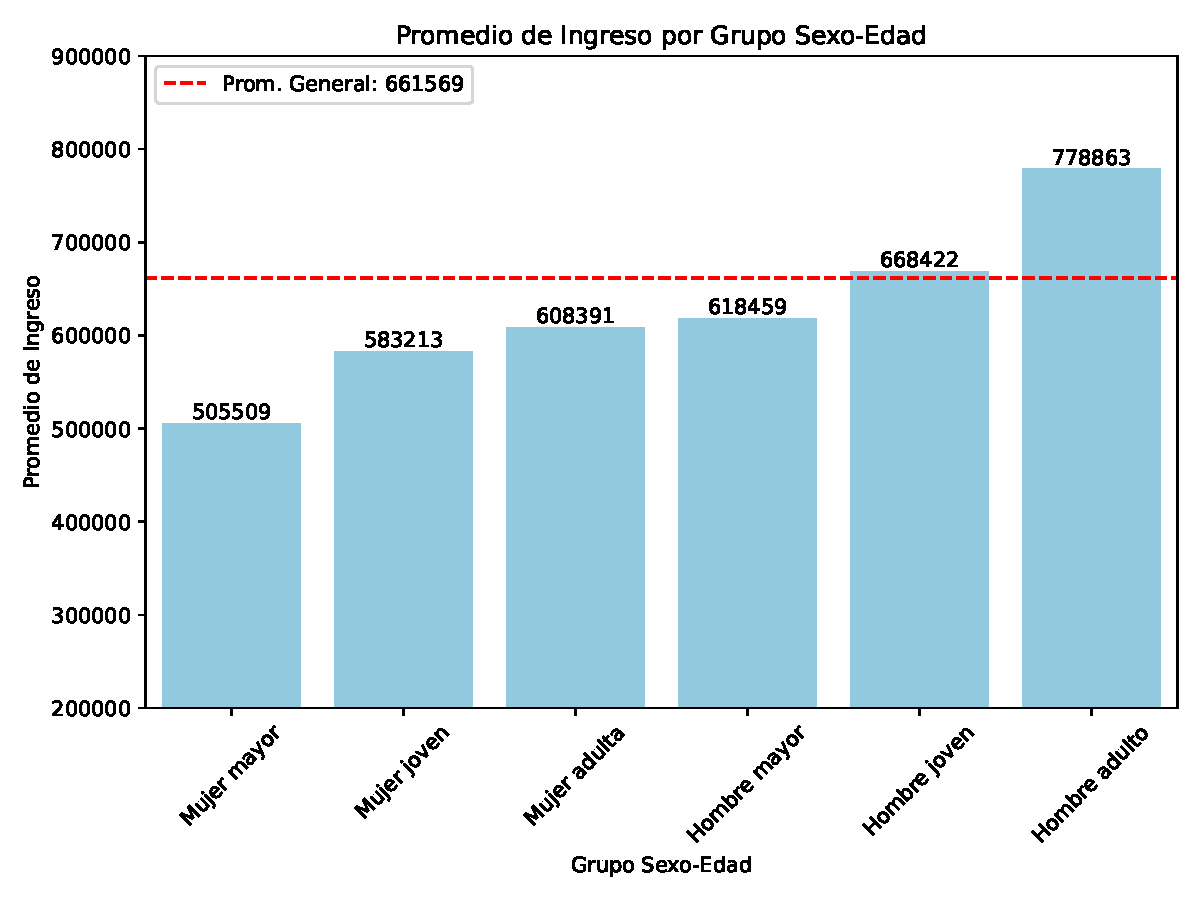
\includegraphics[width=1\textwidth]{../output/fig/PromIngSexoEdad.pdf}
	% 		\caption{\label{5a} Sexo y Edad}
	% 	\end{subfigure}
	% 	\hfill
	% 	\begin{subfigure}[b]{0.49\textwidth}
	% 		\centering
	% 		\includegraphics[width=1\textwidth]{../output/fig/PromIngEduca.pdf}
	% 		\caption{\label{5b} Nivel Educacional}
	% 	\end{subfigure}
	% 	\caption{Promedio de Ingresos por Sexo, Edad y Nivel Educacional}
	% 	\label{05fig}
	% \end{figure}
	
	% \FloatBarrier

% \section{Conclusiones}



%\printbibliography

\addcontentsline{toc}{chapter}{\textbf{Bibliografía}} 
\lhead{Bibliografía}
\renewcommand{\bibname}{Bibliografía}

% \bibliographystyle{unsrt}
% \begin{thebibliography}{9}

\bibliographystyle{apacite}
\bibliography{Referencias}

% \end{thebibliography}

\end{document}
